\section{Description séquentielle des modules}
    \label{sec:modules}
    
Le diagramme de séquence présenté dans cette section a pour objectif d'illustrer le fonctionnement des trois principales fonctionnalités de Glasir : le Filtre, l'Optimiseur et l'Editeur de fonction. Pour rappel, la lecture d'un diagramme de séquence se fait de haut en bas suivant un ordre chronologique, et en suivant les flèches. Les flèches correpondent aux méthodes des différentes classes présentées en tête du diagramme, l'éxecution d'une fonction est représentée par une barre verticale sur la colonne de la classe correspondante. Une fonction est appelée et rend une valeur en retour, et peut appeler d'autres fonctions lors de son éxecution.

	    \begin{figure}[H]
	        \centering
	        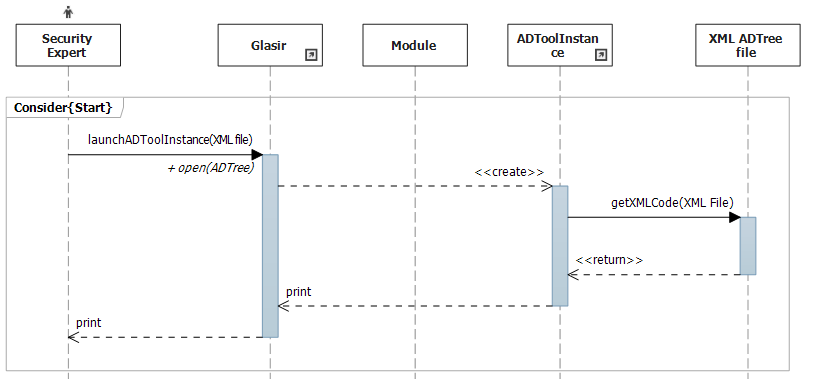
\includegraphics[height=0.45\textwidth]{figure/startseqdiag.png}
	        \caption{Diagramme de séquence du démarrage d'une instance d'ADTool dans Glasir.}
	        \label{fig:start}
	    \end{figure}

Dans un but de synthèse, nous avons représenté le diagramme de séquence du fonctionnement d'un module, pouvant représenter n'importe laquelle des fonctionnalités de Glasir. Les différences entre chaque module sont détaillées plus loin dans cette section. Pour mieux saisir le fonctionnement de l'un de ces modules, la {\sc Figure}~{\ref{fig:start}} illustre l'ouverture d'un ADTree dans Glasir : l'expert en sécurité demande à ouvrir un fichier XML contenant un ADTree dans Glasir. Ce dernier crée alors une instance d'ADTool, qui va chercher le code XML du fichier afin d'afficher l'ADTree.

	    La {\sc Figure}~{\ref{fig:moduleseq}} illustre le fonctionnement générique d'un module. L'expert en sécurité spécifie d'abord les paramètres de l'opération que va effectuer le module. Puis, une fois lancé, le module va effectuer des opérations sur le fichier de l'ADTree cible. Un fichier résultat au format XML est alors généré puis ouvert dans une nouvelle instance d'ADTool, afin d'être affiché à l'écran. 

	    \begin{figure}[H]
	        \centering
			\hspace*{-1.2cm}
	        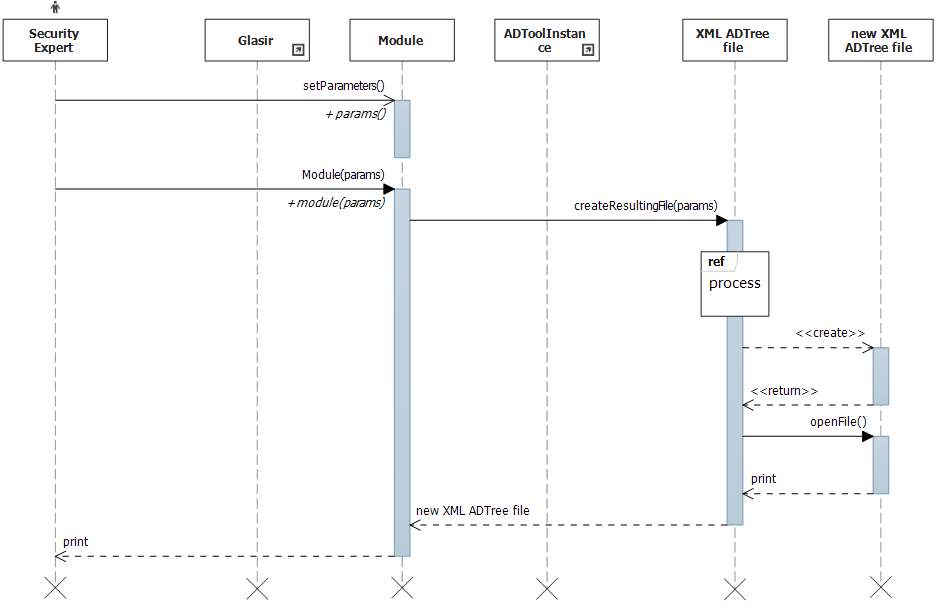
\includegraphics[height=0.75\textwidth]{figure/moduleSeqDiag.png}
	        \caption{Diagramme de séquence générique d'un module.}
	        \label{fig:moduleseq}
	    \end{figure}

Le bloc nommé \og process \fg{} illustre la partie différente de chaque module, tout le reste (ouverture du module avec les paramètres , et création et ouverture du fichier résultat) étant commun à tous les modules.

Dans le cas du Filtre, les paramètres passés à l'appel sont les intervalles\footnote{ADTool propose des paramètres de valuation tels que le coût d'une attaque (un nombre réel) ou sa faisabilité (un booléen). Bien que certains de ces paramètres soient définis sur un ensemble discret, il est toujours possible de définir une relation d'ordre sur cet ensemble, et donc d'y définir des intervalles.} de filtrage sur les valuations de l'ADTree. Le bloc process réalise l'algorithme de filtrage, qui a déjà été présenté dans le rapport de spécifications fonctionnelles~\cite{spec_fonc}, appliqué au contenu du fichier XML de l'ADTreer.

En ce qui concerne l'Editeur de fonctions, les paramètres passés à l'appel sont la formule de calcul du paramètre à définir, et son nom. Le bloc process contient la série de calculs nécessaires à l'attribution des valeurs du nouveaux paramètres à chacun des noeuds de l'ADTree.  

Enfin, le paramètre passé lors de l'appel de l'Optimiseur désigne le paramètre de valuation de l'ADTree selon lequel l'expert veut réaliser l'optimisation. Le bloc process réalise l'algorithme d'optimisation sur le contenu du fichier XML de l'ADTree, algorithme qui a déjà été détaillé dans le rapport de spécifications fonctionnelles~\cite{spec_fonc}. 